\section{Описание раздела <<Клиенты>>}\label{sec:sec14_1}
\begin{enumerate}[\thesection .1]
\item Раздел позволяет работать со списком точек ТП.
В модуле выполняются следующие операции:
\begin{itemize}
	\item Просмотр списка клиентов;
	\item Просмотр детальной информации по клиенту;
	\item Просмотр детальной информации по юридическому лицу клиента;
	\item Добавление выбранного клиента в текущий маршрут ТП.
	\item Добавление нового клиента;
%	\item Создание события для клиента.
\end{itemize}
\item Основное окно модуля содержит список точек. В каждом элементе списка содержится название точки и ее адрес. 
%Добавить картинку
\item Добавление ТТ в маршрут
Чтобы добавить точку в маршрут необходимо:
\begin{itemize}
	\item Произвести длительное касание на наименовании соответствующей ТТ;
	\item В открывшемся информационном окне для подтверждения операции добавления ТТ в маршрут нажать кнопку «Да». После чего точка будет добавлена в маршрут на текущую дату;\footnote{Точки, добавленные маршрут, выделяются в списке жирным курсивом.}
\end{itemize}

\item Окно просмотра информации о ТТ
При касании элемента в списке в основном окне модуля "Клиенты" происходит переход в окно просмотра детальной информации о точке (рис.\ref{pic:pic14_1}). В окне отображается следующая информация: 
\begin{itemize}
	\item Клиент;
	\item Адрес;
	\item Телефон;
	\item Контактное лицо;
	\item Комментарий;
	\item Юр. лицо (при касании происходит переход в окно просмотра информации о юр.лице);
	\item дополнительные атрибуты точки;	
\end{itemize}
\begin{figure}[!h]
	\begin{floatrow}
		\ffigbox{\caption{Окно просмотра информации о ТТ}\label{pic:pic14_1}}%
		{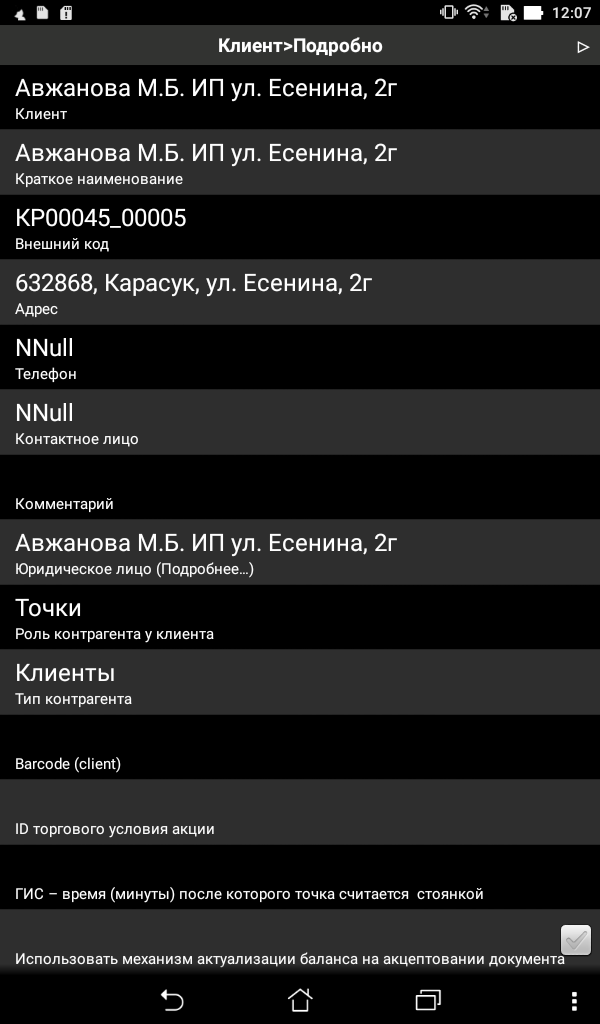
\includegraphics[width=0.8\linewidth]{scr14_1.png}}
		\ffigbox{\caption{Выделение клиентов с просроченными задолженностями}\label{pic:pic14_2}}%
		{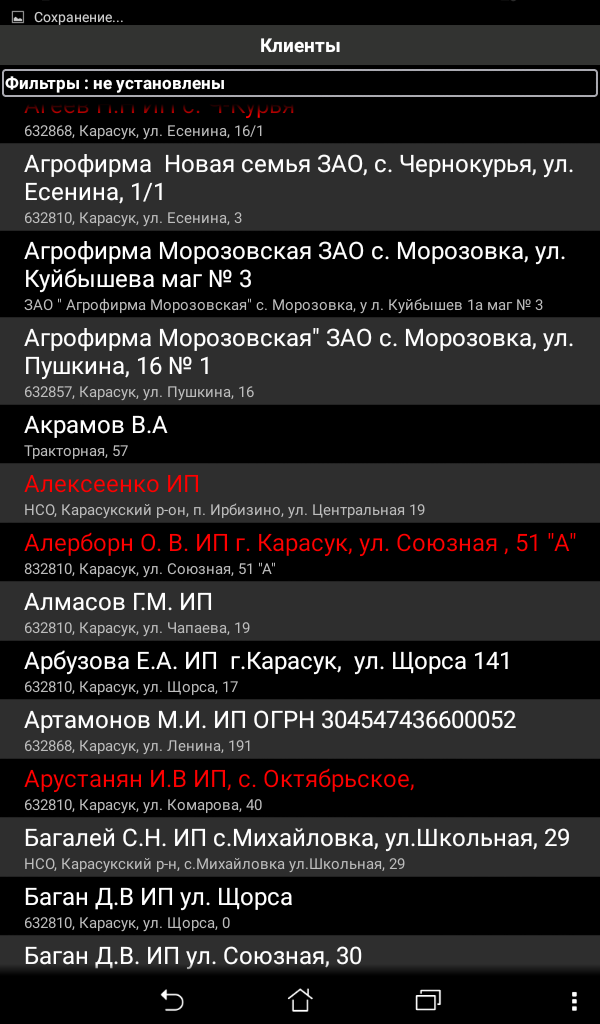
\includegraphics[width=0.8\linewidth]{scr14_2.png}}         
	\end{floatrow}
\end{figure}
\item Выделение клиентов с просроченными задолженностями
В Системе предусмотрено выделение записи о клиенте красным цветом в случае, если у клиента имеется просроченная задолженность.(рис.\ref{pic:pic14_2})
\end{enumerate}